
\noindent\textbf{Solución 1}\\\\

Por datos 

\begin{equation} \label{eq_51M4_shg00100019_0}
	\mid\overline{AB}\mid + \mid\overline{CD}\mid = \mid\overline{AD}\mid + \mid\overline{BC}\mid
\end{equation}

Sean

\begin{equation} \label{eq_51M4_shg00100019_1}
	I := bisector(\angle DCB) \cap bisector(\angle ABC)
\end{equation}
\begin{equation} \label{eq_51M4_shg00100019_2}
	\sigma := circle(I, d(I, AB))
\end{equation}

Como $I$ equidista de $\overline{AB}$, $\overline{BC}$ y $\overline{CD}$ entonces 

\begin{equation} \label{eq_51M4_shg00100019_3}
	\labelcref{eq_51M4_shg00100019_1}, \labelcref{eq_51M4_shg00100019_2} \vdash \forall l \in \{\overline{AB}, \overline{BC}, \overline{CD} \}\ \mid \sigma \cap l \mid = 1
\end{equation}

Es decir $\sigma$ es tangente a $\overline{AB}$, $\overline{BC}$ y $\overline{CD}$. Por tanto es posible definir los puntos de contacto de la manera siguiente:

\begin{equation} \label{eq_51M4_shg00100019_4}
\begin{gathered}
	\sigma \cap \overline{AB} = \{A'\} \\
	\sigma \cap \overline{BC} = \{B'\} \\
	\sigma \cap \overline{CD} = \{C'\}
\end{gathered}
\end{equation}

Es preciso constatar inicialmente que 

\begin{equation} \label{eq_51M4_shg00100019_5}
	\labelcref{eq_51M4_shg00100019_3}, \labelcref{eq_51M4_shg00100019_4} \vdash (\mid\overline{BA'}\mid = \mid\overline{BB'})\mid \land (\mid\overline{CB'}\mid = \mid\overline{CC'}\mid)
\end{equation}

Como $A'$ , $B'$, $C'$ son puntos interiores de los respectivos lados de $ABCD$ se cumple que

\begin{equation} \label{eq_51M4_shg00100019_6}
\begin{gathered}
	\mid\overline{AA'}\mid + \mid\overline{BA'}\mid = \mid\overline{AB}\mid \\
	\mid\overline{BB'}\mid + \mid\overline{CB'}\mid = \mid\overline{BC}\mid \\
	\mid\overline{CC'}\mid + \mid\overline{DC'}\mid = \mid\overline{CD}\mid
\end{gathered}
\end{equation}

... y combinado esto con los datos del problema

\begin{equation} \label{eq_51M4_shg00100019_7}
	\labelcref{eq_51M4_shg00100019_0}, \labelcref{eq_51M4_shg00100019_6} \vdash \mid\overline{AA'}\mid + \mid\overline{DC'}\mid = \mid\overline{DA}\mid
\end{equation}

Tracemos entonces la tangente desde $D$ a $\sigma$ en $D'$ hasta que se intercepte con $AB$ en el punto $A\textsubscript{1}$ , es decir

\begin{equation} \label{eq_51M4_shg00100019_8}
	(A\textsubscript{1} \in AB) \land (\sigma \cap A\textsubscript{1}D = \{D'\})\\
\end{equation}

Como consecuencia 

\begin{equation} \label{eq_51M4_shg00100019_9}
\begin{gathered}
	 \labelcref{eq_51M4_shg00100019_8}, \labelcref{eq_51M4_shg00100019_4} \vdash (\mid\overline{A\textsubscript{1}D'}\mid = \mid\overline{A\textsubscript{1}A'}\mid) \land (\mid\overline{DD'}\mid = \mid\overline{DC'}\mid)
\end{gathered}
\end{equation}

\begin{equation} \label{eq_51M4_shg00100019_9a}
	\mid\overline{DA\textsubscript{1}}\mid = \mid DD'\mid + \mid D'A \mid
\end{equation}

Se pueden dar tres casos . Si $A\textsubscript{1} = A$ entonces el problema tiene solución evidente. Quedan entonces otras dos opciones.

El primer caso se fundamenta en suponer que

\begin{equation} \label{eq_51M4_shg00100019_10}
	\sigma \cap AD = \emptyset
\end{equation}

Entonces 

\begin{equation} \label{eq_51M4_shg00100019_11}
	\labelcref{eq_51M4_shg00100019_10} \vdash A\textsubscript{1} \in \overline{AA'}
\end{equation}
\begin{equation} \label{eq_51M4_shg00100019_12}
	\labelcref{eq_51M4_shg00100019_11} \vdash \mid\overline{AA\textsubscript{1}}\mid = \mid\overline{AA'}\mid - \mid\overline{A\textsubscript{1}A'}\mid
\end{equation}
\begin{equation} \label{eq_51M4_shg00100019_13}
	\labelcref{eq_51M4_shg00100019_7}, \labelcref{eq_51M4_shg00100019_9}, \labelcref{eq_51M4_shg00100019_12} \vdash \mid\overline{AA\textsubscript{1}}\mid + \mid\overline{A\textsubscript{1}D}\mid = \mid\overline{AD}\mid
\end{equation}

En el segundo caso corresponde suponer que

\begin{equation} \label{eq_51M4_shg00100019_14}
	\sigma \cap AD \neq \emptyset
\end{equation}

Entonces 

\begin{equation} \label{eq_51M4_shg00100019_15}
	\labelcref{eq_51M4_shg00100019_14} \vdash A \in \overline{A\textsubscript{1}A}
\end{equation}
\begin{equation} \label{eq_51M4_shg00100019_16}
	\labelcref{eq_51M4_shg00100019_15} \vdash \mid\overline{AA\textsubscript{1}}\mid + \mid\overline{AA'}\mid = \mid\overline{A\textsubscript{1}A'}\mid
\end{equation}
\begin{equation} \label{eq_51M4_shg00100019_17}
	\labelcref{eq_51M4_shg00100019_7}, \labelcref{eq_51M4_shg00100019_9}, \labelcref{eq_51M4_shg00100019_16} \vdash \mid\overline{AA\textsubscript{1}}\mid + \mid\overline{AD}\mid = \mid\overline{A\textsubscript{1}D}\mid
\end{equation}

En ambos casos se incumple la desigualdad triangular. Por esta razón la única opción posible es $A = A\textsubscript{1}$

\vspace{1cm}
Lo que queda demostrado. \\\\\\

\noindent\textbf{Solución 2}\\\\

Sabemos que 
\begin{equation}
\label{eq1}
|AB| + |CD| = |AD| + |BC|
\end{equation}

\begin{center}
	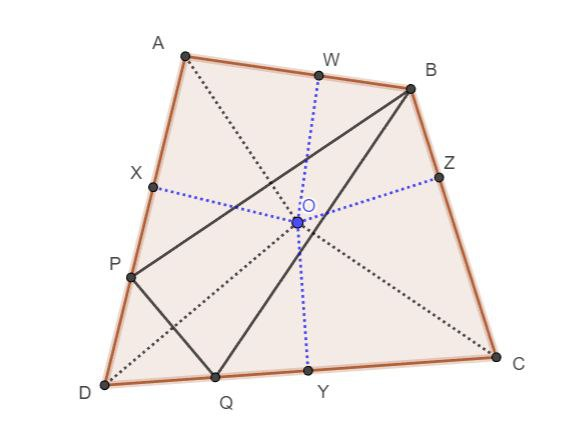
\includegraphics[width=0.8\textwidth]{img/51M04_shg00100019.1.png}
\end{center}

Sin pérdida de generalidad supongamos que $AB < AD$ y tomemos $P\in AD$ tal que $AP = AB$. De \eqref{eq1} sabemos que $DP < DC$ así que podemos tomar $Q\in DC$ tal que $PD =DQ$. Ahora, \eqref{eq1} implica que $QC ) CB$. Veamos que los triángulos $\triangle  ABP, \triangle DPQ, \triangle CQB$ son isósceles de donde las bisectrices de los ángulos $\angle  PAB, \angle QDP, \angle BCQ$ se intersectan en el circuncentro $O$ del $\triangle BPQ$.

Si $W,X,Y,Z$ son las proyecciónes de $O$ sobre los lados del cuadrilátero se concluye notando que $\triangle OAW = \triangle OAX \Rightarrow OW = OX$, análogamente $OX = OY = OZ$ por tanto la circunferencia con centro $O$ y radio $OW$ es tangente a los 4 lados del cuadrilátero.